\documentclass[11pt,a4paper]{article}
\usepackage[utf8]{inputenc}
\usepackage[vietnamese]{babel}
\usepackage{amsmath,amssymb}
\usepackage[version=4]{mhchem}
\usepackage{geometry}
\geometry{top=1.5cm,bottom=1.2cm,left=1.4cm,right=1.4cm,headheight=28pt,headsep=12pt,footskip=18pt}
\usepackage{graphicx}
\usepackage{xcolor}
\usepackage{tabularx}
\usepackage{array}
\usepackage{tikz}
\usepackage{multicol}
\usepackage{fancyhdr}
\usepackage{enumitem}

\definecolor{hfRed}{HTML}{D32F2F}
\definecolor{hfGreen}{HTML}{8BC390}
\definecolor{mainGreen}{HTML}{2E7D32}

\usepackage{ex_test}
\bracketExpl{true}

\pagestyle{fancy}
\fancyhf{}
\renewcommand{\headrulewidth}{0.75pt}
\renewcommand{\headrule}{\hbox to\headwidth{\color{hfGreen}\leaders\hrule height \headrulewidth\hfill}}
\renewcommand{\footrulewidth}{0.75pt}
\renewcommand{\footrule}{\hbox to\headwidth{\color{hfGreen}\leaders\hrule height \footrulewidth\hfill}}

\fancyhead[L]{\small\itshape\color{hfRed}Tài liệu lưu hành nội bộ}
\fancyhead[R]{\small\color{hfRed}Thầy \textbf{TRẦN VĂN THẠNH} - 0777.470.803}

\fancyfoot[L]{\footnotesize\itshape\color{hfRed}CS1: 6/15 Nguyễn Hoàng, P. Kim Long, TP Huế \quad|\quad CS2: 24 Đặng Thái Thân, TP Huế}
\fancyfoot[R]{\small\textbf{\color{hfRed}Trang \thepage}}

\setlength{\parindent}{0pt}
\setlength{\parskip}{1.5pt}

\def\loigiai#1{
\par\begingroup\color{blue!80!black}\small
\noindent\textbf{\textit{Lời giải chi tiết:}}\par
#1\par\endgroup}

\begin{document}

\Opensolutionfile{ans}[ans-de08-gv]

\noindent
\begin{minipage}[t]{0.48\textwidth}
	\centering
	\textbf{SỞ GIÁO DỤC VÀ ĐÀO TẠO THỪA THIÊN HUẾ}\\
	\textbf{ĐỀ CHÍNH THỨC}\\
	\textit{(Đề thi có 04 trang)}
\end{minipage}\hfill
\begin{minipage}[t]{0.48\textwidth}
	\centering
	\textbf{\color{mainGreen}ĐỀ KIỂM TRA ĐỊNH KỲ CHƯƠNG 3 (HỢP CHẤT NITROGEN)}\\
	\textbf{MÔN: HOÁ HỌC -- LỚP 12}\\
	\textit{Thời gian làm bài: 50 phút (không kể thời gian phát đề)}\\
	\textbf{Mã đề thi: 108}
\end{minipage}


\vspace{0.1cm}
\begin{center}
	\textbf{\color{hfRed}\Large (BẢN GIÁO VIÊN -- CÓ LỜI GIẢI CHI TIẾT)}
\end{center}

\vspace{0.1cm}
\noindent\textit{Họ, tên thí sinh: \dots\dots\dots\dots\dots\dots\dots\dots\dots\dots\dots\dots\dots\dots\dots\dots\dots\dots\dots\dots\dots\dots Lớp: \dots\dots\dots\dots SBD: \dots\dots\dots\dots}\\
\noindent\textit{(Cho biết nguyên tử khối: H = 1; C = 12; N = 14; O = 16; Na = 23; S = 32; Cl = 35,5; Fe = 56; Cu = 64).}

\vspace{0.15cm}
\noindent
\textbf{PHẦN I (4,5 điểm -- 18 câu): Câu trắc nghiệm nhiều phương án lựa chọn.}\\
\textit{Thí sinh trả lời từ câu 1 đến câu 18. Mỗi câu hỏi thí sinh chỉ chọn một phương án.}

\setcounter{ex}{0}

\begin{ex}
(SBT -- KNTT). Amine nào sau đây ở trạng thái lỏng ở nhiệt độ phòng?
\choice
{Methylamine}
{Ethylamine}
{Dimethylamine}
{\True Aniline}
\loigiai{
Ở điều kiện thường, methylamine, dimethylamine, trimethylamine và ethylamine là chất khí có mùi khai khó chịu, độc, tan nhiều trong nước.\\
Aniline (\ce{C6H5NH2}) là chất lỏng, sôi ở 184 $^\circ$C, không màu, rất độc, ít tan trong nước, nặng hơn nước.\\
\textbf{Chọn D.}}
\end{ex}

\begin{ex}
Khi alkylamine bậc một phản ứng với nitrous acid (\ce{HNO2}) qua phương trình sau:\\
\centerline{\ce{RNH2 + HNO2 -> ROH + N2 + H2O} \quad (R: gốc alkyl)}\\
Trong phản ứng trên thì alkylamine đóng vai trò là chất
\choice
{oxi hóa}
{base}
{\True khử}
{acid}
\loigiai{
Trong phân tử alkylamine \ce{RNH2}, nguyên tử nitrogen có số oxi hóa $-3$ tăng lên 0 trong \ce{N2}.\\
Nitrous acid (\ce{HNO2}) chứa N($+3$) giảm xuống 0 trong \ce{N2}.\\
Do đó, alkylamine đóng vai trò là chất khử, còn \ce{HNO2} là chất oxi hóa.\\
\textbf{Chọn C.}}
\end{ex}

\begin{ex}
Trong phân tử amine: N còn một cặp e chưa liên kết nên có thể tạo ra liên kết \dots\dots\dots\dots\dots (giống \ce{NH3}) do đó các amine có tính chất hóa học tương tự ammonia.
{\centering
	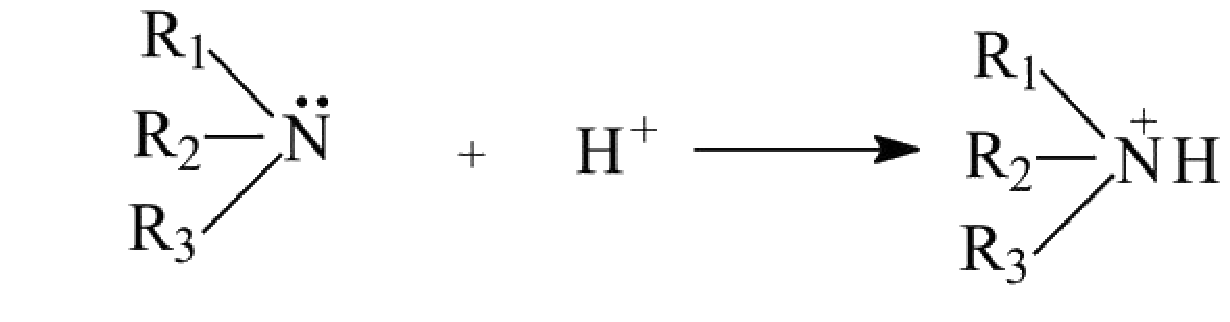
\includegraphics[width=6.0cm]{images_crop_de08/cau03_amine_hplus.png}\par}
Cụm từ điền vào khoảng trống là
\choice
{\True cho nhận}
{ion}
{cộng hóa trị thường}
{hydrogen}
\loigiai{
Cặp electron tự do chưa liên kết trên nguyên tử nitrogen của amine có thể nhường vào orbital trống của ion \ce{H+} để tạo liên kết phối trí (liên kết cho - nhận), tương tự như phân tử ammonia \ce{NH3}. Do đó amine thể hiện tính base.\\
\textbf{Chọn A.}}
\end{ex}

\begin{ex}
Chất nào sau đây là amino acid?
\choice
{Acid glutaric}
{\True Acid glutamic}
{Glycerol}
{Aniline}
\loigiai{
Glutamic acid (\ce{HOOC-CH2-CH2-CH(NH2)-COOH}) là một amino acid (axit 2-aminopentanedioic).\\
Glutaric acid là dicarboxylic acid; Glycerol là polyalcohol; Aniline là arylamine.\\
\textbf{Chọn B.}}
\end{ex}

\begin{ex}
(SBT -- KNTT). Quá trình di chuyển của các amino acid trong điện trường được gọi là
\choice
{\True sự điện di}
{sự điện li}
{sự điện phân}
{sự điện giải}
\loigiai{
Sự điện di (electrophoresis) là hiện tượng chuyển động của các hạt mang điện (như ion, amino acid, protein) dưới tác dụng của một điện trường ngoài.\\
\textbf{Chọn A.}}
\end{ex}

\begin{ex}
(SBT -- CTST). Amino acid \textbf{không} có loại phản ứng nào sau đây?
\choice
{Phản ứng với acid và base}
{Phản ứng ester hoá}
{Phản ứng trùng ngưng}
{\True Phản ứng thủy phân}
\loigiai{
Amino acid là hợp chất đơn phân tử chứa đồng thời nhóm chức carboxyl (-\ce{COOH}) và amino (-\ce{NH2}), không chứa liên kết peptide hay liên kết ester nên không tham gia phản ứng thủy phân. Phản ứng thủy phân là đặc trưng của peptide, protein, ester\dots\\
\textbf{Chọn D.}}
\end{ex}

\begin{ex}
Số liên kết peptide trong hợp chất pentapeptide là
\choice
{3}
{\True 4}
{5}
{6}
\loigiai{
Pentapeptide là peptide được tạo nên từ 5 gốc $\alpha$-amino acid, do đó số liên kết peptide bằng $5 - 1 = 4$.\\
\textbf{Chọn B.}}
\end{ex}

\begin{ex}
(SBT -- KNTT). Loại liên kết được hình thành giữa các amino acid trong peptide được gọi là
\choice
{liên kết ion}
{liên kết hydrogen}
{\True liên kết peptide}
{liên kết cộng hoá trị}
\loigiai{
Liên kết peptide (-\ce{CO-NH}-) là liên kết amide được hình thành giữa nhóm carboxyl của một $\alpha$-amino acid với nhóm amino của một $\alpha$-amino acid khác.\\
\textbf{Chọn C.}}
\end{ex}

\begin{ex}
Protein hình cầu tan được trong nước tạo dung dịch keo như
\choice
{$\alpha$-keratin (ở tóc, móng)}
{Collagen (ở da, sụn)}
{\True Albumin (lòng trắng trứng)}
{Myosin (ở cơ bắp)}
\loigiai{
Albumin trong lòng trắng trứng là protein dạng hình cầu, tan được trong nước tạo dung dịch keo.\\
Keratin, collagen, myosin là protein dạng hình sợi không tan trong nước.\\
\textbf{Chọn C.}}
\end{ex}

\begin{ex}
Ứng dụng nào sau đây \textbf{không} phải là của protein?
\choice
{\True Là thành phần tạo nên chất dẻo}
{Là thành phần cấu tạo tế bào}
{Là cơ sở tạo nên sự sống}
{Là dinh dưỡng thức ăn}
\loigiai{
Protein đóng vai trò cấu trúc tế bào, vận chuyển chất và cung cấp dinh dưỡng thiết yếu cho cơ thể sống. Protein không được dùng để chế tạo chất dẻo (nhựa polymer công nghiệp).\\
\textbf{Chọn A.}}
\end{ex}



\begin{ex}
(SBT -- CTST). Trong dãy các chất sau đây, tính base của amine thể hiện qua phản ứng với các chất:
\choice
{\True \ce{HCl}, \ce{H2SO4}, \ce{CuCl2}}
{\ce{Cl2}, \ce{H2SO4}, \ce{FeCl3}}
{\ce{NaOH}, \ce{HCl}, \ce{FeCl3}}
{\ce{O2}, \ce{HCl}, \ce{CuCl2}}
\loigiai{
Tính base của amine thể hiện qua phản ứng với acid vô cơ (\ce{HCl}, \ce{H2SO4} tạo muối ammonium) và phản ứng tạo kết tủa hydroxide/phức chất với dung dịch muối (\ce{CuCl2}, \ce{FeCl3}). Dãy B có \ce{Cl2} (chất oxi hóa), dãy C có \ce{NaOH} (base), dãy D có \ce{O2}. Dãy phù hợp nhất là \ce{HCl}, \ce{H2SO4}, \ce{CuCl2}.\\
\textbf{Chọn A.}}
\end{ex}

\begin{ex}
(SBT -- CTST). Cơ thể người mã hoá được loại amino acid nào sau đây trong tổng hợp protein cho cơ thể?
{\centering
	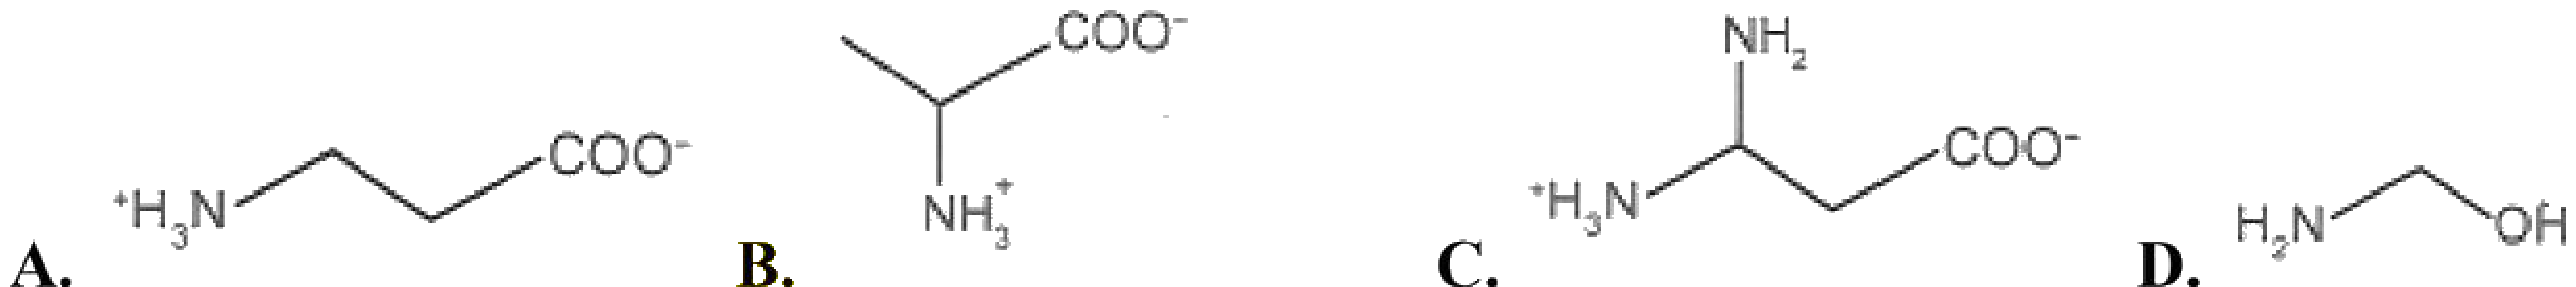
\includegraphics[width=13.5cm]{images_crop_de08/cau12_options.png}\par}
\choice
{Cấu tạo A}
{\True Cấu tạo B}
{Cấu tạo C}
{Cấu tạo D}
\loigiai{
Protein của cơ thể người được tạo nên từ 20 loại $\alpha$-amino acid chuẩn do mã di truyền trực tiếp mã hóa.\\
Công thức ở phương án B là \ce{CH3-CH(NH3+)-COO-} (alanine) là $\alpha$-amino acid.\\
Phương án A ($\beta$-alanine) và C ($\gamma$-aminobutyric acid / GABA) không tham gia cấu tạo protein theo mã di truyền.\\
\textbf{Chọn B.}}
\end{ex}

\begin{ex}
(SBT -- KNTT). Trong phản ứng của amine với \ce{Cu(OH)2}, sản phẩm có màu xanh đặc trưng là do
\choice
{\True sự tạo phức giữa \ce{Cu^2+} và -\ce{NH2}}
{sự oxi hoá \ce{Cu^2+} khi gặp amine}
{phản ứng giữa \ce{OH-} và -\ce{NH2}}
{giải phóng \ce{H2} khi phản ứng}
\loigiai{
Các alkylamine đơn giản dùng cặp electron tự do trên nguyên tử N tạo liên kết phối trí với ion \ce{Cu^2+}, hình thành ion phức $\ce{[Cu(RNH2)4]^2+}$ có màu xanh lam đặc trưng.\\
\textbf{Chọn A.}}
\end{ex}

\begin{ex}
(SBT -- CTST). Cơ thể người sử dụng phân tử nào sau đây để xây dựng protein?
\choice
{Tinh bột}
{Chất béo}
{\True Amino acid}
{Acid béo}
\loigiai{
Amino acid là các đơn phân (monomer) để cơ thể tổng hợp nên các chuỗi polypeptide và phân tử protein.\\
\textbf{Chọn C.}}
\end{ex}

\begin{ex}
(SBT -- CTST). Các hợp chất amine, amino acid, peptide và protein có nhóm chức chung nào sau đây?
\choice
{Carboxyl}
{Amide}
{Ammonium}
{\True Amine hoặc amino}
\loigiai{
Nhóm chức chứa nguyên tố nitrogen có mặt xuyên suốt trong các phân tử amine, amino acid, peptide và protein là nhóm amine (hoặc amino: -\ce{NH2}, -\ce{NH}-, =\ce{N}-).\\
\textbf{Chọn D.}}
\end{ex}

\begin{ex}
Amine và amino acid nào sau đây có cùng bậc?
\choice
{Dimethylamine và alanine}
{Dimethylamine và glutamic acid}
{\True Dimethylamine và proline}
{Trimethylamine và lysine}
\loigiai{
Dimethylamine (\ce{(CH3)2NH}) là amine bậc 2.\\
Proline là amino acid vòng có nhóm amino bậc 2 (-\ce{NH}- gắn với 2 nguyên tử C trong khung dị vòng pyrrolidine).\\
Do đó dimethylamine và proline có cùng bậc 2.\\
\textbf{Chọn C.}}
\end{ex}

\begin{ex}
(SBT -- CTST). Tính chất hoá học của methylamine và alanine đều có
\choice
{phản ứng với ninhydrin}
{phản ứng thuỷ phân}
{\True phản ứng với dung dịch \ce{HCl}}
{phản ứng với dung dịch \ce{NaOH}}
\loigiai{
Cả methylamine (\ce{CH3NH2}) và alanine (\ce{CH3CH(NH2)COOH}) đều có nhóm amino mang tính base nên đều phản ứng được với dung dịch acid \ce{HCl} tạo muối ammonium.\\
Methylamine không phản ứng với \ce{NaOH}, không có phản ứng màu ninhydrin.\\
\textbf{Chọn C.}}
\end{ex}

\begin{ex}
Cho các phát biểu sau:\\
(a) Trong dung dịch, glycine tồn tại chủ yếu ở dạng ion lưỡng cực.\\
(b) Amino acid là chất rắn kết tinh, dễ tan trong nước.\\
(c) Phản ứng thế bromine vào vòng thơm của aniline dễ hơn benzene.\\
(d) Hợp chất \ce{H2N-CH2-COO-CH3} tác dụng được với dung dịch \ce{NaOH} và dung dịch \ce{HCl}.\\
(e) Triolein và protein có cùng thành phần nguyên tố.\\
(g) Trong phân tử, các amino acid đều chỉ có một nhóm \ce{NH2} và một nhóm \ce{COOH}.\\
Số phát biểu đúng là
\choice
{\True 4}
{5}
{3}
{6}
\loigiai{
(a) Đúng, trong dung dịch glycine tồn tại chủ yếu ở dạng ion lưỡng cực $\ce{^+H3N-CH2-COO-}$.\\
(b) Đúng, amino acid tồn tại dạng ion lưỡng cực tương tự hợp chất ion nên là chất rắn kết tinh, nhiệt độ nóng chảy cao và dễ tan trong nước.\\
(c) Đúng, nhóm -\ce{NH2} đẩy electron làm tăng mật độ electron trong nhân thơm, phản ứng thế \ce{Br2} xảy ra dễ dàng hơn benzene tạo kết tủa trắng.\\
(d) Đúng, methyl glycinate vừa có nhóm -\ce{NH2} (tác dụng với \ce{HCl}) vừa có nhóm ester (bị thủy phân bởi \ce{NaOH}).\\
(e) Sai, triolein chứa C, H, O còn protein bắt buộc có C, H, O, N.\\
(g) Sai, amino acid có thể có nhiều nhóm -\ce{NH2} hoặc nhiều nhóm -\ce{COOH} (ví dụ Lysine có 2 nhóm \ce{NH2}, Glutamic acid có 2 nhóm \ce{COOH}).\\
=> Có 4 phát biểu đúng: (a), (b), (c), (d).\\
\textbf{Chọn A.}}
\end{ex}

\Closesolutionfile{ans}



\vspace{0.15cm}
\noindent
\textbf{PHẦN II (4,0 điểm -- 4 câu): Câu trắc nghiệm đúng sai.}\\
\textit{Thí sinh trả lời từ câu 1 đến câu 4. Trong mỗi ý a), b), c), d) ở mỗi câu, thí sinh chọn đúng hoặc sai.}

\setcounter{ex}{0}

\begin{ex}
(SBT -- KNTT). Các phát biểu về tính chất hoá học của dung dịch aniline:
\choiceTF
{\False Dung dịch aniline làm quỳ tím chuyển sang màu xanh}
{\True Dung dịch aniline tạo kết tủa trắng khi thêm vào nước bromine}
{\True Aniline phản ứng với \ce{HCl} tạo phenylammonium chloride}
{\True Aniline phản ứng với \ce{HNO2} tạo muối phenyldiazonium}
\loigiai{
a) Sai. Do ảnh hưởng hút electron của nhân benzene, tính base của aniline rất yếu không làm đổi màu quỳ tím.\\
b) Đúng. $\ce{C6H5NH2 + 3Br2 -> C6H2Br3NH2 v + 3HBr}$ (kết tủa trắng 2,4,6-tribromoaniline).\\
c) Đúng. $\ce{C6H5NH2 + HCl -> C6H5NH3Cl}$ (phenylammonium chloride).\\
d) Đúng. Ở $0 - 5\ ^\circ\text{C}$: $\ce{C6H5NH2 + HNO2 + HCl -> [C6H5N2]+Cl- + 2H2O}$.\\
\textbf{Đáp án: a - S, b - Đ, c - Đ, d - Đ.}}
\end{ex}

\begin{ex}
(SBT -- CTST). Cho một số hợp chất chứa nguyên tố nitrogen như hình bên dưới:\\
{\centering
	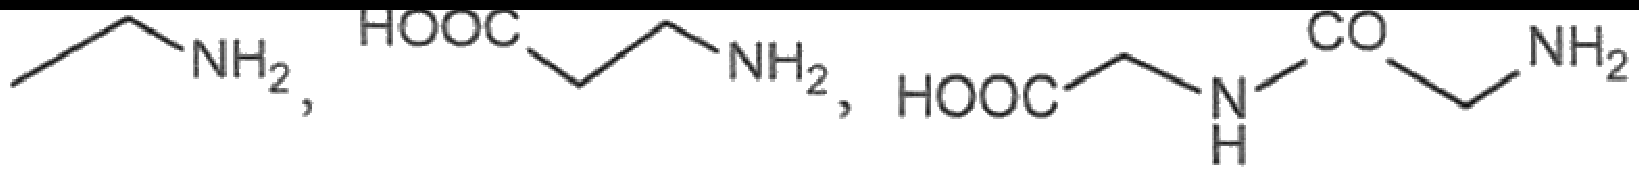
\includegraphics[width=11.5cm]{images_crop_de08/p2_cau2_compounds.png}\par}
Về phân loại hợp chất và đặc điểm cấu tạo, xét tính đúng/sai của các phát biểu sau:
\choiceTF
{\True Có 1 hợp chất hữu cơ thuộc loại amine}
{\False Có 2 hợp chất hữu cơ thuộc loại amino acid}
{\False Có 1 hợp chất hữu cơ đơn chức, 2 hợp chất tạp chức, 3 hợp chất chứa nhóm $\alpha$-\ce{NH2}}
{\True Trong 3 hợp chất trên chỉ có 1 liên kết peptide}
\loigiai{
Chất (1) là ethylamine \ce{CH3-CH2-NH2} (amine đơn chức).\\
Chất (2) là $\beta$-alanine \ce{H2N-CH2-CH2-COOH} (amino acid tạp chức, nhóm -\ce{NH2} ở vị trí $\beta$).\\
Chất (3) là dipeptide Gly-Ala \ce{H2N-CH2-CONH-CH(CH3)-COOH} (tạp chức, có 1 liên kết peptide và nhóm $\alpha$-\ce{NH2} ở đầu N).\\
a) Đúng. Chỉ có chất (1) là amine.\\
b) Sai. Chỉ có chất (2) là amino acid; chất (3) là dipeptide.\\
c) Sai. Chất (2) có nhóm $\beta$-\ce{NH2}, chất (1) không có nhóm carboxyl, chỉ có chất (3) có nhóm $\alpha$-\ce{NH2}. Vậy không có 3 hợp chất chứa nhóm $\alpha$-\ce{NH2}.\\
d) Đúng. Chỉ có dipeptide (3) chứa đúng 1 liên kết peptide -\ce{CONH}-.\\
\textbf{Đáp án: a - Đ, b - S, c - S, d - Đ.}}
\end{ex}

\begin{ex}
Acetyl Hexapeptide-8 là một hợp chất peptide. Chất này được biết đến là một thành phần có khả năng liên kết với nước để phục hồi da và là một chất dẫn truyền thần kinh làm giảm nếp nhăn hình thành do lão hóa hoặc bởi các biểu hiện thay đổi trên cơ mặt gây ra.
{\centering
	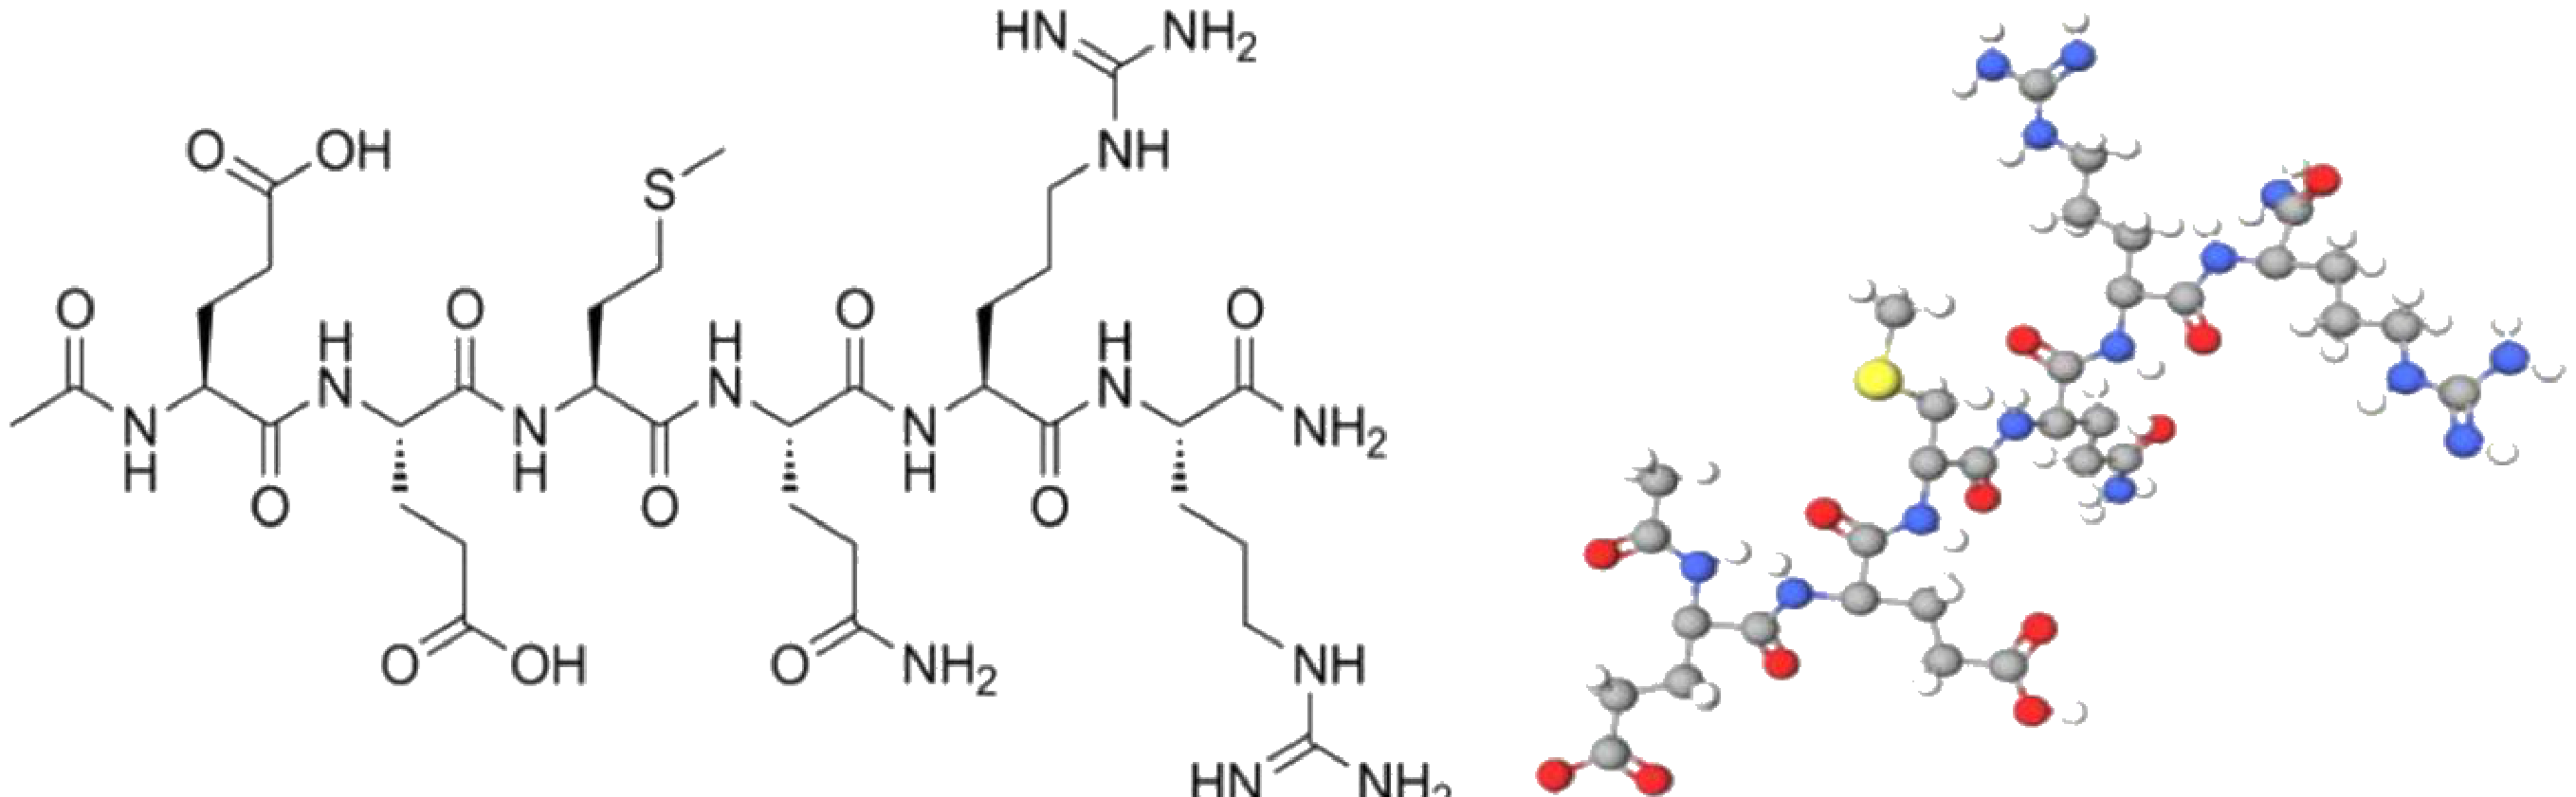
\includegraphics[width=12.5cm]{images_crop_de08/p2_cau3_acetyl_hexapeptide.png}\par}
\choiceTF
{\False Acetyl Hexapeptide-8 là một hợp chất amino acid}
{\False Acetyl Hexapeptide-8 có chứa các nguyên tố C, H, N, O}
{\True Acetyl Hexapeptide-8 là một peptide}
{\True Acetyl Hexapeptide-8 là một hợp chất tạp chức}
\loigiai{
a) Sai. Acetyl Hexapeptide-8 là một hexapeptide biến tính (oligopeptide 6 gốc), không phải amino acid đơn phân.\\
b) Sai. Nhìn vào công thức cấu tạo, phân tử có chứa gốc methionine (-\ce{CH2-CH2-S-CH3}), do đó có chứa thêm nguyên tố lưu huỳnh (S), không chỉ gồm C, H, N, O.\\
c) Đúng. Đây là một hexapeptide có 5 liên kết peptide trong mạch.\\
d) Đúng. Phân tử chứa đồng thời nhiều loại nhóm chức: amide (-\ce{CONH}-), carboxyl (-\ce{COOH}), thioether (-\ce{S}-), hydroxyl (-\ce{OH})\dots nên là hợp chất tạp chức.\\
\textbf{Đáp án: a - S, b - S, c - Đ, d - Đ.}}
\end{ex}

\begin{ex}
Casein là loại protein chủ yếu có trong sữa. Casein là một dạng protein (đạm) có trong sữa mẹ, sữa bò và sữa dê. Vì là protein hoàn chỉnh nên casein bổ sung nhiều amino acid thiết yếu và các hợp chất khác giúp cơ thể tăng trưởng, phát triển.
{\centering
	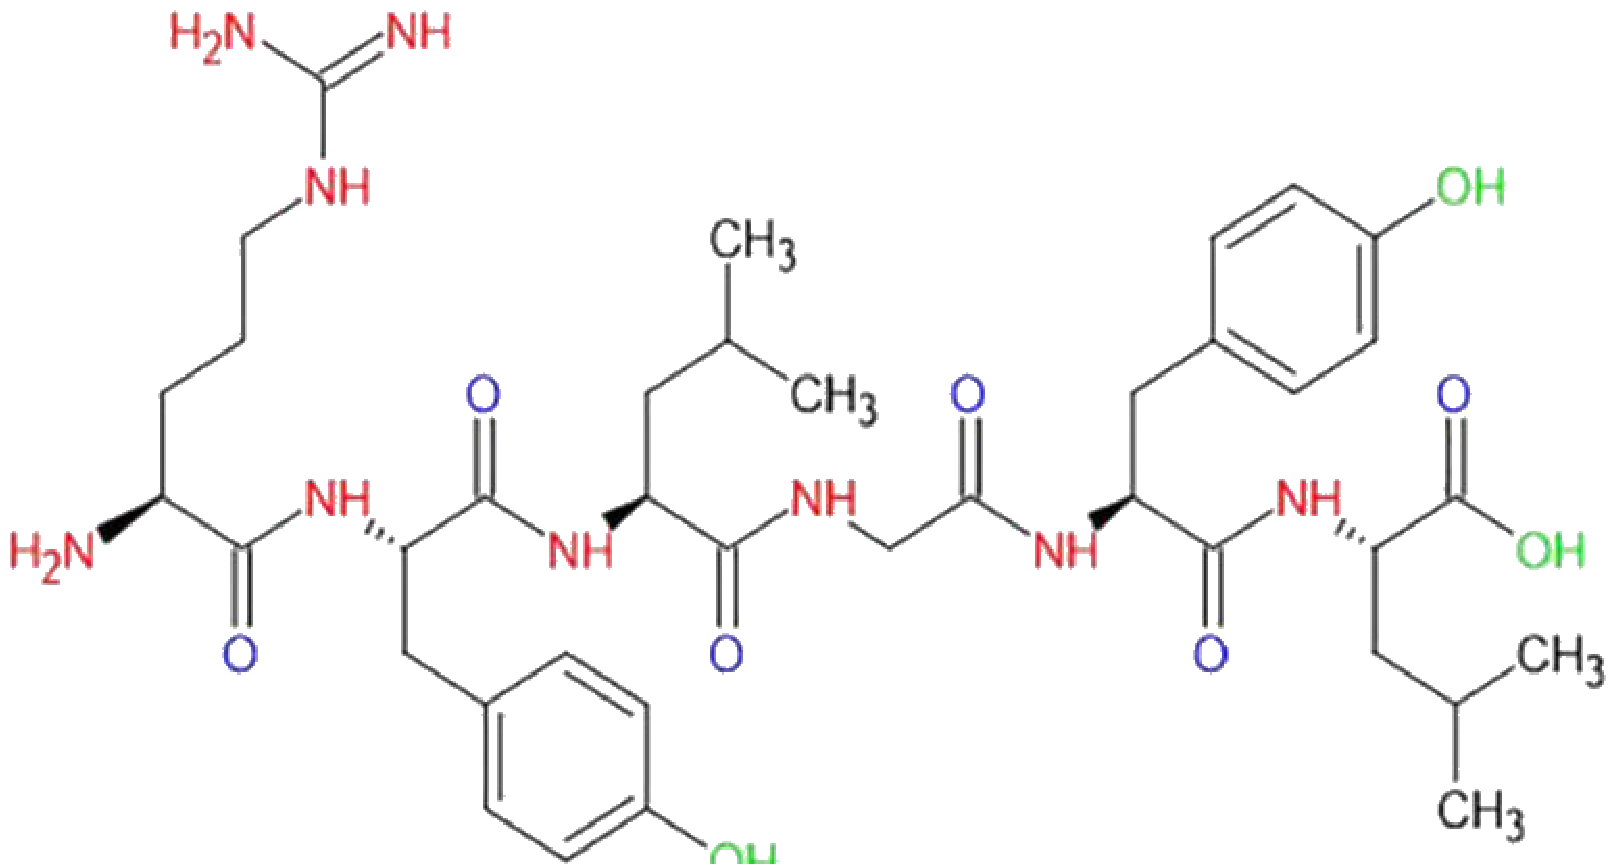
\includegraphics[width=9.5cm]{images_crop_de08/p2_cau4_casein.png}\par}
\choiceTF
{\False Casein là loại protein tan tốt trong nước}
{\True Uống sữa giúp giảm bớt nguy hiểm khi bị ngộ độc bởi muối chì, muối thuỷ ngân}
{\True Vì casein là một loại protein sẽ đông tụ và tách khỏi dung dịch khi thêm dung dịch acid, base, muối của các kim loại nặng như chì, thủy ngân,\dots{} nên uống sữa khi bị ngộ độc muối chì, muối thủy ngân sẽ tạo thành kết tủa và thải được ra ngoài}
{\False Casein là loại protein có duy nhất trong sữa}
\loigiai{
a) Sai. Casein là phosphoprotein hầu như không tan trong nước tinh khiết ở điểm đẳng điện ($pH \approx 4{,}6$); trong sữa, casein tồn tại ở dạng hạt keo micelle phân tán.\\
b) Đúng. Sữa chứa hàm lượng protein cao (đặc biệt là casein) có khả năng kết tủa ion kim loại nặng.\\
c) Đúng. Protein casein đông tụ liên kết với các ion kim loại nặng (\ce{Pb^2+}, \ce{Hg^2+}) tạo kết tủa bền không tan, ngăn ngừa chất độc ngấm qua niêm mạc ruột vào máu.\\
d) Sai. Trong sữa ngoài casein (khoảng 80\%) còn có whey protein (chiếm khoảng 20\%, gồm lactoglobulin, lactalbumin\dots), nên casein không phải protein duy nhất.\\
\textbf{Đáp án: a - S, b - Đ, c - Đ, d - S.}}
\end{ex}



\vspace{0.15cm}
\noindent
\textbf{PHẦN III (1,5 điểm -- 6 câu): Câu trắc nghiệm yêu cầu trả lời ngắn.}\\
\textit{Thí sinh trả lời từ câu 1 đến câu 6. Mỗi câu hỏi thí sinh điền câu trả lời vào ô tương ứng.}

\setcounter{ex}{0}

\begin{ex}
Cho ethylamine lần lượt vào dung dịch \ce{FeCl3}; dung dịch \ce{HCl}; \ce{Cu(OH)2}; dung dịch \ce{NaCl}; dung dịch \ce{Br2}. Ethylamine phản ứng được với bao nhiêu chất?
\loigiai{
Ethylamine (\ce{CH3CH2NH2}) tác dụng được với 3 chất:\\
- Dung dịch \ce{FeCl3}: $\ce{3CH3CH2NH2 + FeCl3 + 3H2O -> Fe(OH)3 v (nâu đỏ) + 3CH3CH2NH3Cl}$.\\
- Dung dịch \ce{HCl}: $\ce{CH3CH2NH2 + HCl -> CH3CH2NH3Cl}$.\\
- \ce{Cu(OH)2}: Hòa tan kết tủa tạo phức xanh lam: $\ce{Cu(OH)2 + 4CH3CH2NH2 -> [Cu(CH3CH2NH2)4](OH)2}$.\\
Ethylamine không phản ứng với dung dịch \ce{NaCl} và dung dịch \ce{Br2}.\\
\textbf{Đáp số: 3.}}
\end{ex}


\begin{ex}
Cho dãy các dung dịch: acetic acid, phenylammonium chloride, sodium acetate, methylamine, glycine, phenol. Số dung dịch trong dãy tác dụng được với dung dịch \ce{NaOH} là
\loigiai{
Các dung dịch tác dụng được với dung dịch \ce{NaOH} gồm:\\
(1) Acetic acid: $\ce{CH3COOH + NaOH -> CH3COONa + H2O}$.\\
(2) Phenylammonium chloride: $\ce{C6H5NH3Cl + NaOH -> C6H5NH2 + NaCl + H2O}$.\\
(3) Glycine: $\ce{H2N-CH2-COOH + NaOH -> H2N-CH2-COONa + H2O}$.\\
(4) Phenol: $\ce{C6H5OH + NaOH -> C6H5ONa + H2O}$.\\
Sodium acetate và methylamine không phản ứng với \ce{NaOH}.\\
=> Có 4 dung dịch tác dụng được với \ce{NaOH}.\\
\textbf{Đáp số: 4.}}
\end{ex}


\begin{ex}
Cho các chất: phenylammonium chloride, alanine, lysine, glycine, ethylamine. Số chất làm quỳ tím đổi màu là
\loigiai{
Xét sự đổi màu quỳ tím của các dung dịch:\\
- Phenylammonium chloride (\ce{C6H5NH3Cl}): Muối của base rất yếu và acid mạnh -> dung dịch có tính acid làm quỳ tím hóa đỏ (hồng).\\
- Alanine (1 nhóm \ce{NH2}, 1 nhóm \ce{COOH}): Quỳ tím không đổi màu.\\
- Lysine (2 nhóm \ce{NH2}, 1 nhóm \ce{COOH}): Tính base trội hơn -> quỳ tím hóa xanh.\\
- Glycine (1 nhóm \ce{NH2}, 1 nhóm \ce{COOH}): Quỳ tím không đổi màu.\\
- Ethylamine: Tính base mạnh -> quỳ tím hóa xanh.\\
=> Có 3 chất làm đổi màu quỳ tím.\\
\textbf{Đáp số: 3.}}
\end{ex}


\begin{ex}
Cho các phát biểu sau:\\
(1) Dung dịch ethylamine và dung dịch aniline đều làm xanh giấy quỳ tím.\\
(2) Nhỏ từ từ đến dư dung dịch methylamine vào dung dịch copper(II) sulfate, ban đầu thấy xuất hiện kết tủa màu xanh nhạt, sau đó kết tủa tan tạo thành dung dịch màu xanh lam.\\
(3) Cho dung dịch methylamine vào ống nghiệm đựng dung dịch iron(III) chloride thấy xuất hiện kết tủa nâu đỏ.\\
(4) Nhỏ vài giọt dung dịch aniline vào ống nghiệm đựng nước bromine thấy xuất hiện kết tủa trắng.\\
Số phát biểu đúng là
\loigiai{
(1) Sai, aniline có tính base rất yếu không làm đổi màu quỳ tím (chỉ ethylamine làm xanh quỳ tím).\\
(2) Đúng, ban đầu tạo kết tủa \ce{Cu(OH)2}, sau đó tạo phức chất hòa tan $\ce{[Cu(CH3NH2)4]^2+}$ xanh lam thẫm.\\
(3) Đúng, methylamine tạo kết tủa nâu đỏ \ce{Fe(OH)3}: $\ce{3CH3NH2 + FeCl3 + 3H2O -> Fe(OH)3 v + 3CH3NH3Cl}$.\\
(4) Đúng, aniline phản ứng thế với bromine tạo kết tủa trắng 2,4,6-tribromoaniline.\\
=> Có 3 phát biểu đúng: (2), (3), (4).\\
\textbf{Đáp số: 3.}}
\end{ex}


\begin{ex}
Thuốc Paracetamol là một loại thuốc được sử dụng rất nhiều trong y học. Thuốc có tác dụng giảm đau, hạ sốt tuy nhiên ít có tác dụng kháng viêm. Thuốc Paracetamol được tổng hợp từ p-nitrophenol theo sơ đồ phản ứng sau (biết hiệu suất của cả quá trình phản ứng đạt 90\%):
{\centering
	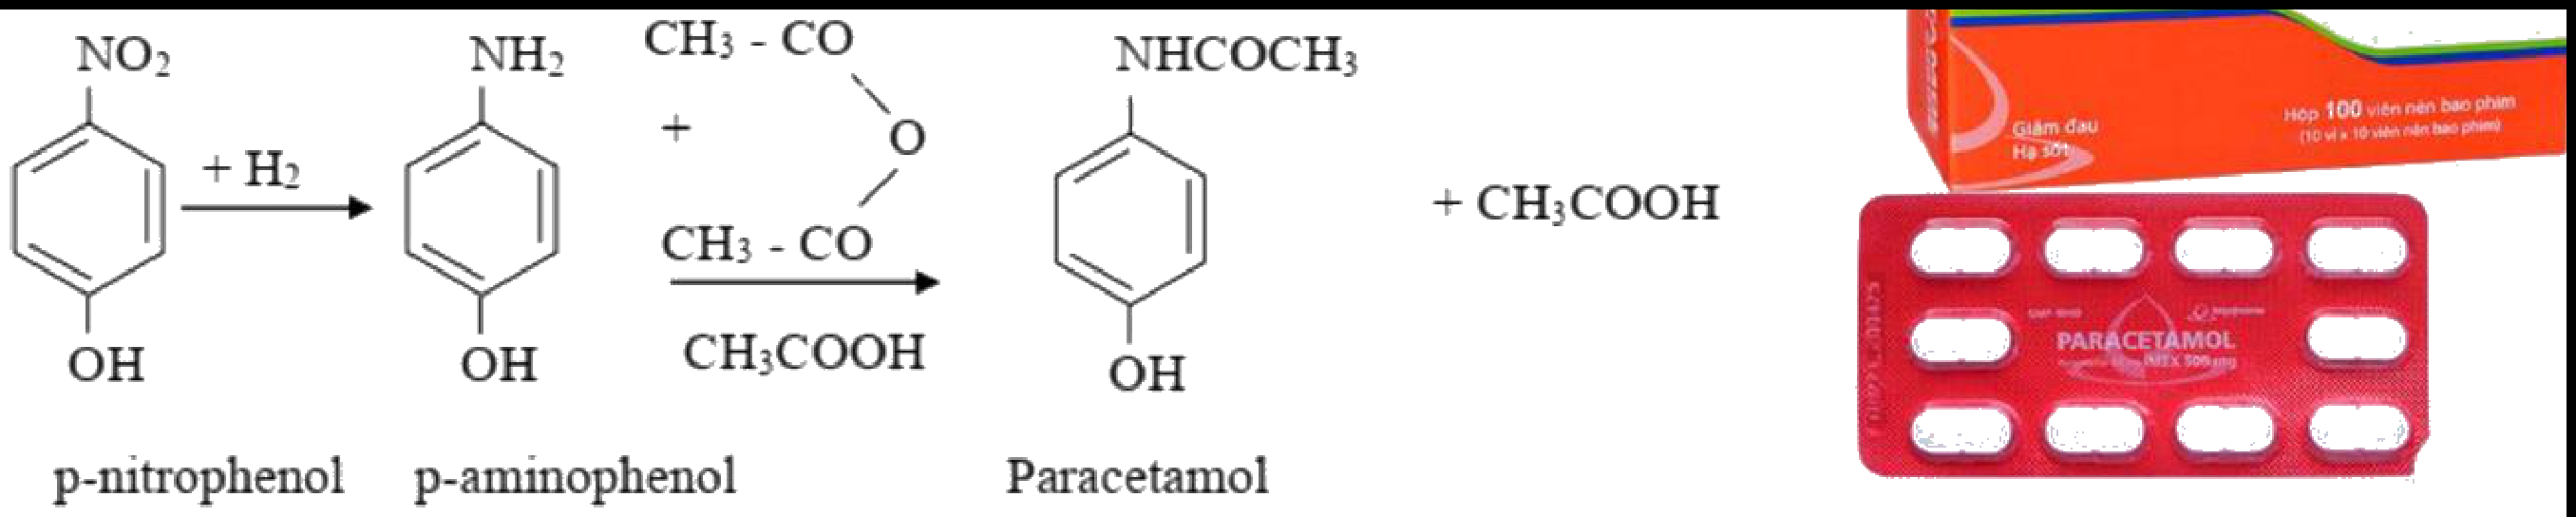
\includegraphics[width=13.0cm]{images_crop_de08/p3_cau5_paracetamol.png}\par}
Để sản xuất 30,2 triệu viên thuốc Paracetamol thì khối lượng p-nitrophenol cần dùng gần nhất với giá trị nào sau đây (theo đơn vị tấn)? Biết rằng mỗi viên thuốc chứa 500 mg Paracetamol.
\loigiai{
Khối lượng mol: $M(\text{Paracetamol}) = 151\ \text{g/mol}$; $M(\text{p-nitrophenol}) = 139\ \text{g/mol}$.\\
Khối lượng Paracetamol cần sản xuất:\\
$m(\text{Paracetamol}) = 30{,}2 \times 10^6 \times 500\ \text{mg} = 30{,}2 \times 10^6 \times 0{,}5\ \text{g} = 15{,}1 \times 10^6\ \text{g} = 15{,}1\ \text{tấn}$.\\
Số mol Paracetamol $= \dfrac{15{,}1 \times 10^6}{151} = 100\,000\ \text{mol}$.\\
Do hiệu suất toàn bộ quá trình đạt 90\%:\\
$n(\text{p-nitrophenol cần dùng}) = \dfrac{100\,000}{0{,}9} \approx 111\,111{,}1\ \text{mol}$.\\
Khối lượng p-nitrophenol cần dùng là:\\
$m = \dfrac{100\,000}{0{,}9} \times 139 \approx 15\,444\,444\ \text{g} \approx 15{,}44\ \text{tấn}$ (hoặc 15,4 tấn).\\
\textbf{Đáp số: 15,44.}}
\end{ex}


\begin{ex}
Một người trưởng thành cần tiêu thụ khoảng 0,8 gram protein cho mỗi kg trọng lượng cơ thể mỗi ngày. Một người nặng 70 kg cần bổ sung bao nhiêu gram protein trong một ngày? Nếu mỗi quả trứng chứa khoảng 6 gram protein, người đó cần ăn bao nhiêu quả trứng để đáp ứng lượng protein cần thiết trong ngày? Biết số quả trứng là một con số chẵn.
\loigiai{
Lượng protein cần thiết cho người nặng 70 kg trong 1 ngày:\\
$m(\text{protein}) = 70 \times 0{,}8 = 56\ \text{gam}$.\\
Số quả trứng cần ăn tương ứng:\\
Số trứng $= \dfrac{56}{6} \approx 9{,}33\ \text{quả}$.\\
Vì cần đáp ứng đủ lượng protein và số quả trứng là số chẵn, nên người đó cần ăn 10 quả trứng.\\
\textbf{Đáp số: 10.}}
\end{ex}


\vspace{0.1cm}
\begin{center}
	\textbf{---------- HẾT ----------}
\end{center}

\vspace{0.3cm}
\noindent
\textbf{\large\color{mainGreen}BẢNG TỔNG HỢP ĐÁP ÁN ĐỀ SỐ 08}

\vspace{0.2cm}
\noindent\textbf{PHẦN I:}\\
\begin{tabular}{|c|c|c|c|c|c|c|c|c|c|c|c|c|c|c|c|c|c|}
\hline
\textbf{1} & \textbf{2} & \textbf{3} & \textbf{4} & \textbf{5} & \textbf{6} & \textbf{7} & \textbf{8} & \textbf{9} & \textbf{10} & \textbf{11} & \textbf{12} & \textbf{13} & \textbf{14} & \textbf{15} & \textbf{16} & \textbf{17} & \textbf{18} \\
\hline
D & C & A & B & A & D & B & C & C & A & A & B & A & C & D & C & C & A \\
\hline
\end{tabular}

\vspace{0.3cm}
\noindent\textbf{PHẦN II:}\\
\begin{tabular}{|c|c|c|c|c|}
\hline
\textbf{Câu} & \textbf{Lệnh hỏi a} & \textbf{Lệnh hỏi b} & \textbf{Lệnh hỏi c} & \textbf{Lệnh hỏi d} \\
\hline
\textbf{1} & S & Đ & Đ & Đ \\
\hline
\textbf{2} & Đ & S & S & Đ \\
\hline
\textbf{3} & S & S & Đ & Đ \\
\hline
\textbf{4} & S & Đ & Đ & S \\
\hline
\end{tabular}

\vspace{0.3cm}
\noindent\textbf{PHẦN III:}\\
\begin{tabular}{|c|c|c|c|c|c|c|}
\hline
\textbf{Câu} & \textbf{1} & \textbf{2} & \textbf{3} & \textbf{4} & \textbf{5} & \textbf{6} \\
\hline
\textbf{Đáp số} & 3 & 4 & 3 & 3 & 15,44 & 10 \\
\hline
\end{tabular}

\end{document}
